\newpage
\subsection{Datenbank}
In folgendem soll Aufschluss über die Struktur der Datenbank des ChatBots gegeben werden.
Die Datenbank wird in einer NoSql mongoDb Datenbank gehalten.

\subsubsection{Datenhaltung}
Die Daten, die in der mongDb Datenbank gespeichert sind, sollen über ein Webinterface verändert werden können.
Wenn der Chatbot gestartet wird lädt der Chatbot den Korpus aus der mongoDb.
Sollten die Daten der Datenbank verändert worden sein, dann muss der Chatbot den Korpus erneut laden.
Damit die Veränderungen der Datenbank auch beim Chatbot geändert werden.

\subsubsection{ER Diagramme}
Hier werden die ER Diagramme für die Datenbank aufgeführt.
Zusätzlich wird erklärt welche Daten bei den Entities enthalten sind.

\begin{figure}[H]
    \centering
    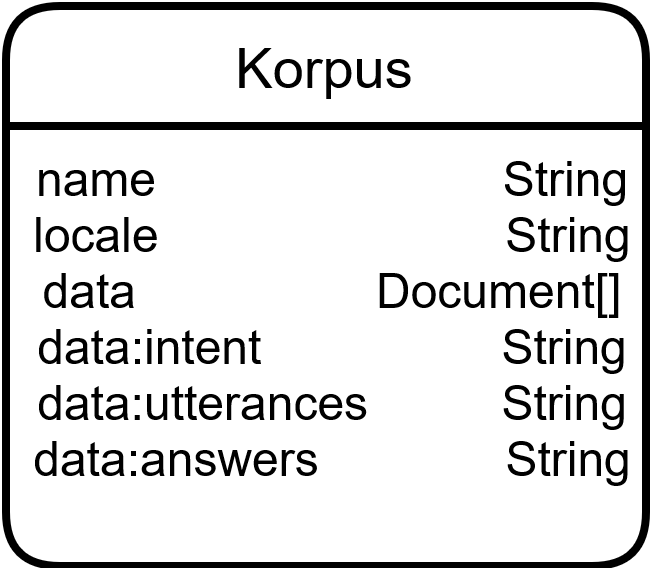
\includegraphics[width=0.5\textwidth]{bilder/technologien/ERMDiagram.png}
    \caption{ER Diagramm Korpus}
    \label{fig:ER_Diagramm_Korpus}
\end{figure}

\noindent Der Korpus besteht aus name, locale und data. 
Der ''name'' ist der Name des Korpus. 
Das ''locale'' gibt an in welcher Sprache der Korpus verfasst wurde. 
Das ''data'' ist gefüllt mit Intents, die benötigt werden, um einschätzen zu können in welchem Kontext der ChatBot antworten soll. 
Der Intent besteht aus Utterances (Äußerung/ Frage des Nutzers) und Antworten. 
Die Utterances sind die möglichen Fragen des Nutzers und die Antworten sind die möglichen Antwortmöglichkeiten des Chatbots. 
Ein Korpus hat sehr viele Intents, die den Wissensschatz des ChatBots abbilden. 

\begin{figure}[H]
    \centering
    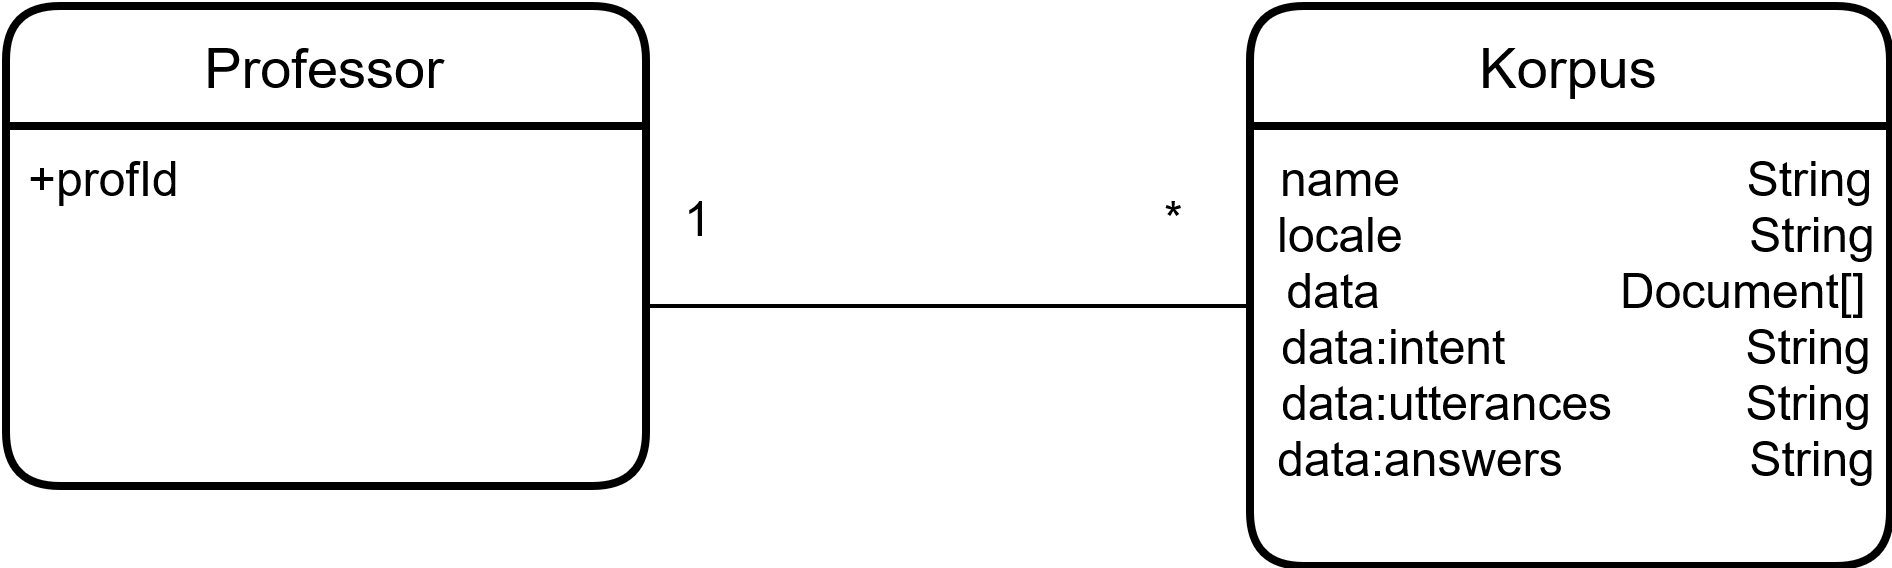
\includegraphics[width=0.8\textwidth]{bilder/technologien/ER-Prof.png}
    \caption{ER Diagramm Professor}
    \label{fig:ER_Diagramm_Professor}
\end{figure}

\noindent In der Abbildung \ref{fig:ER_Diagramm_Professor} soll dargestellt werden, dass ein Professor auf mehrere Korpusse zugreifen kann.
Der Professor wird mit einer ''profID'' ausgestattet, 
damit man bestimmen kann welche Korpusse ihm zugeordnet sind.

\begin{figure}[H]
    \centering
    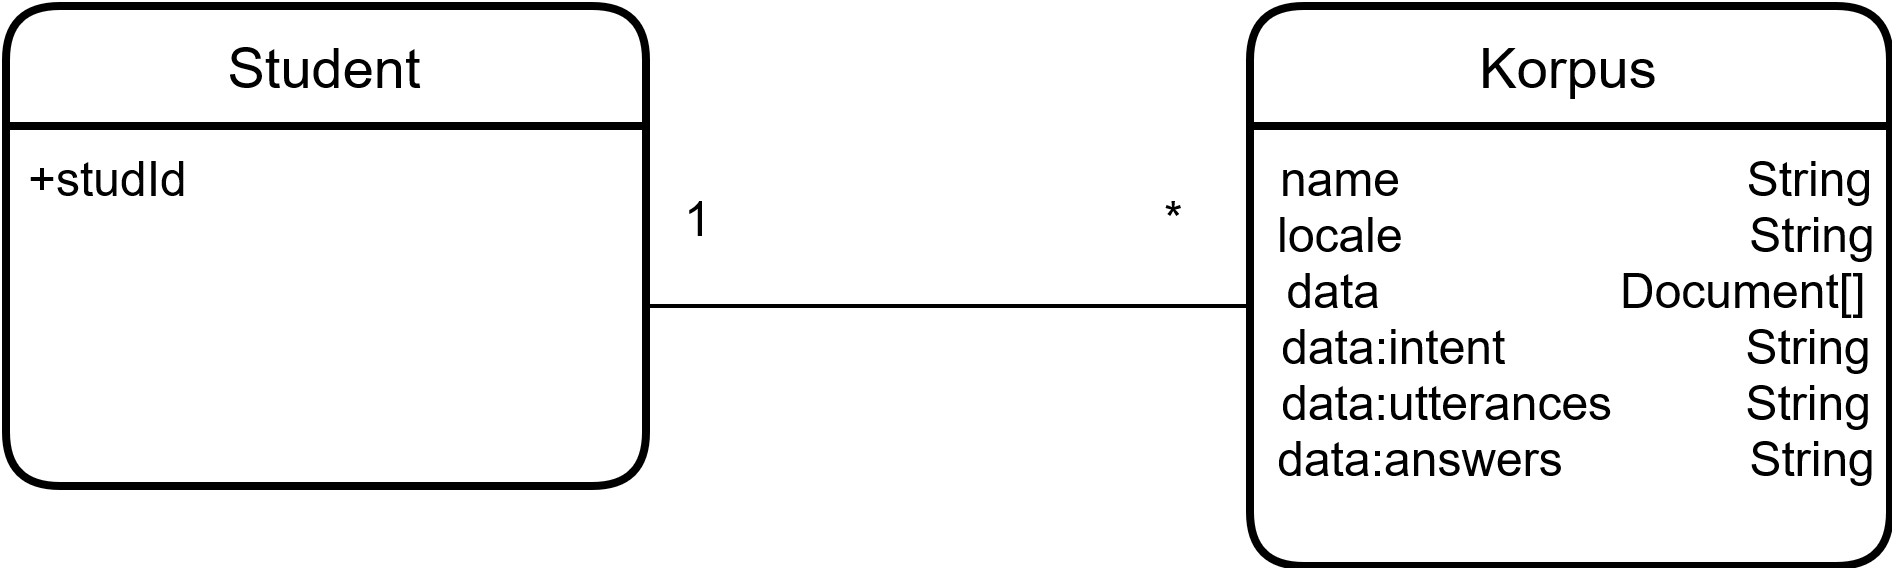
\includegraphics[width=0.8\textwidth]{bilder/technologien/ER-Student.png}
    \caption{ER Diagramm Student}
    \label{fig:ER_Diagramm_Student}
\end{figure}

\noindent In der Abbildung \ref{fig:ER_Diagramm_Student} soll dargestellt werden, dass ein Student auf mehrere Korpusse zugreifen kann.
Der Nutzer bekommt eine ''studId'' damit man bestimmen kann, 
welche Korpusse für den Studenten bereitgestellt werden müssen.

\begin{figure}[H]
    \centering
    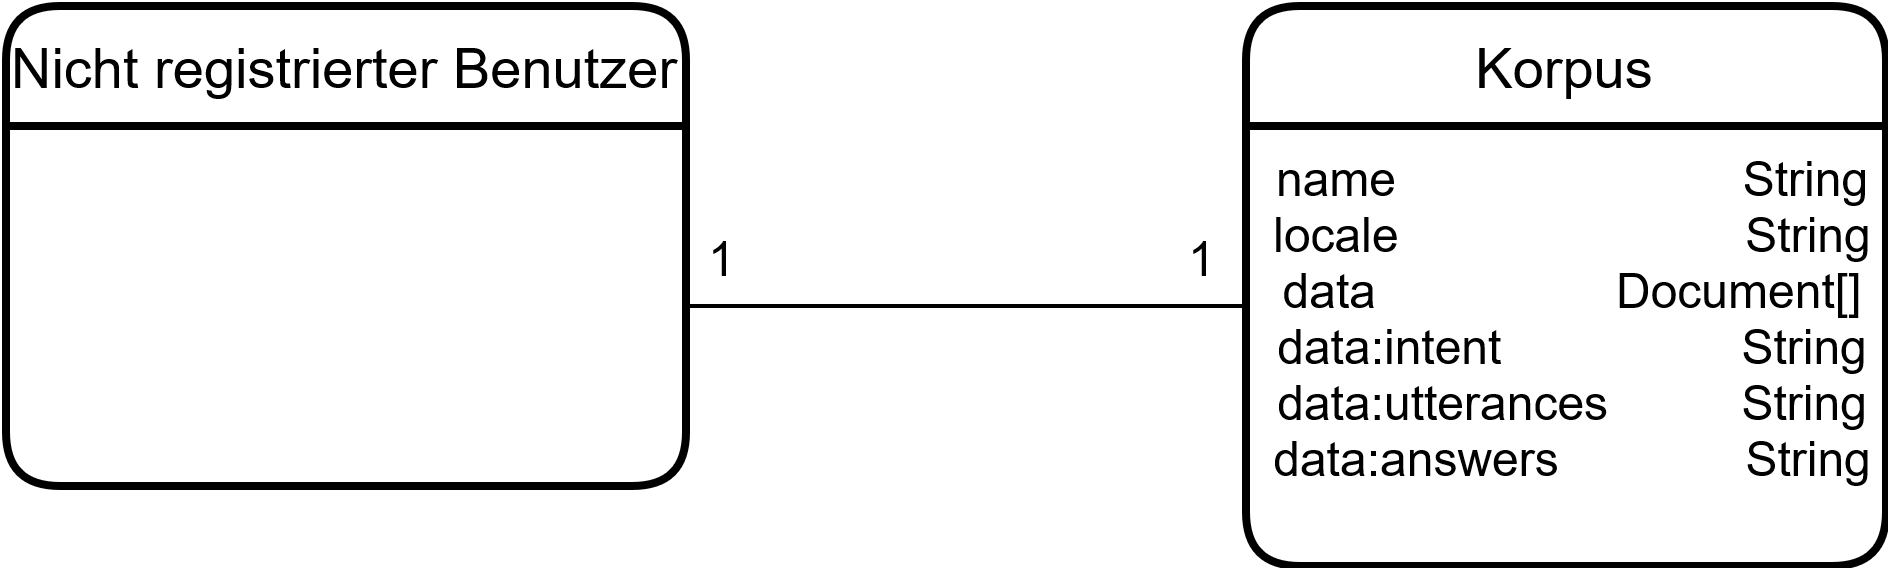
\includegraphics[width=0.8\textwidth]{bilder/technologien/ER-UUser.png}
    \caption{ER Diagramm Unregistrierter Nutzer}
    \label{fig:ER_Diagramm_UUser}
\end{figure}

\noindent In der Abbildung \ref{fig:ER_Diagramm_UUser} soll dargestellt werden, dass ein nicht registrierter Benutzer nur Zugriff auf einen Korpus hat.
Für unregistrierte Benutzer soll nur der Korpus ''Allgemein'' zur Verfügung stehen.
